\documentclass[aspectratio=169,11pt,xcolor=dvipsnames]{beamer}
\usepackage{graphicx} % For including graphics.
\usepackage{hyperref} % For links.
\usepackage{multirow}
\usepackage{minted}

\title{Computer Graphics with Clojure, LWJGL, and Fastmath}
\author{Jan Wedekind}
\date{Saturday, October 18th 2025}

\hypersetup{pdftitle          = {Computer Graphics with Clojure, LWJGL, and Fastmath},
            pdfsubject        = {rendering NASA CGI Moon Kit data using Clojure, LWJGL, and Fastmath},
            pdfauthor         = {Jan Wedekind},
            pdfkeywords       = {Clojure, LWJGL, Fastmath, rendering, NASA, Moon, graphics},
            pdfcreator        = {LaTeX with Beamer class},
            pdfproducer       = {TeX Live 2025/dev/Debian},
            bookmarksopen     = false,
            bookmarksnumbered = true,
            colorlinks        = true,
            filecolor         = cyan,
            citecolor         = green,
            linkcolor         = blue,
            urlcolor          = blue}

\usebackgroundtemplate{
\includegraphics[width=\paperwidth,height=\paperheight]{slide}}

\usecolortheme{seahorse}

\definecolor{slidecolor}{rgb}{0.65,0.71,0.72}
\setbeamercolor{titlelike}{fg=black,bg=slidecolor!60}
\setbeamercolor{frametitle}{fg=black,bg=slidecolor!100}

\begin{document}

\begin{frame}
  \pdfbookmark[1]{Computer Graphics with Clojure, LWJGL, and Fastmath}{title}
  \titlepage{}
\end{frame}

\begin{frame}
  \pdfbookmark[1]{About Me}{bio}
  \frametitle{About Me}
  \begin{minipage}[b]{0.79\textwidth}
    \begin{itemize}
      \item Computer Science at Karlsruhe University
        \begin{itemize}
          \item compiler construction, robotics, measurement engineering
        \end{itemize}
      \item Measurement Engineering at Carl Zeiss SMT AG, Oberkochen
      \item PhD on Computer Vision using Ruby at Sheffield Hallam University
      \item Graphical User Interface Development at Digital Science, London
      \item Computer Vision and Machine Learning at Roke, Romsey
    \end{itemize}
  \end{minipage}
  \begin{minipage}[b]{0.2\textwidth}
    
\includegraphics[width=\textwidth]{avatar}\\
    \begin{tiny}
      \url{https://www.wedesoft.de/}
    \end{tiny}
  \end{minipage}
\end{frame}

\begin{frame}
  \pdfbookmark[1]{Software Libre}{foss}
  \frametitle{Software Libre}
  \begin{itemize}
    \item Anymeal recipe database software
    \item HornetsEye Ruby computer vision software
    \item AIscm GNU Guile extension for numerical arrays and tensors
    \item sfsim space flight simulator
  \end{itemize}
  \bigskip
  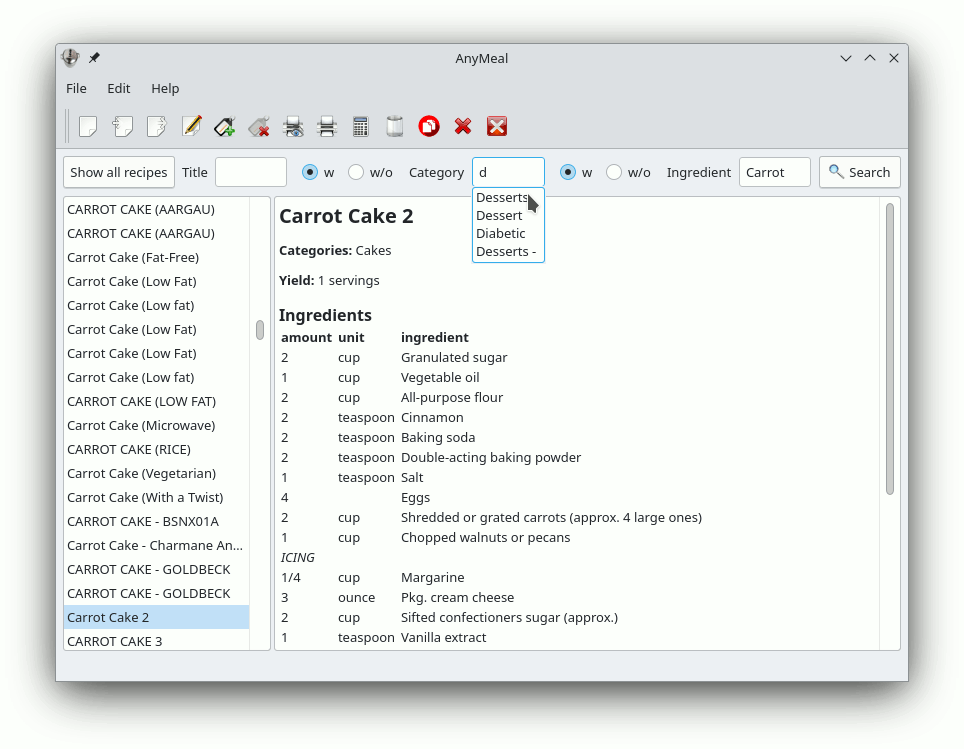
\includegraphics[width=.24\textwidth]{anymeal}
  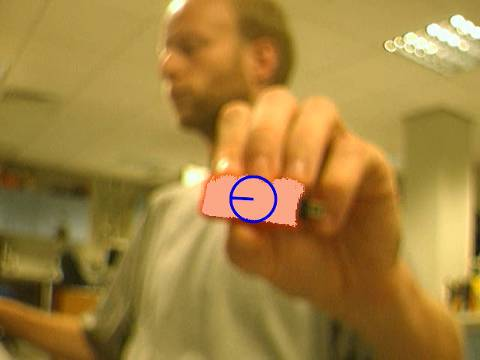
\includegraphics[width=.24\textwidth]{hornetseye}
  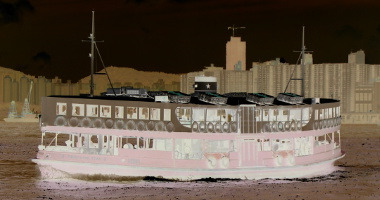
\includegraphics[width=.24\textwidth]{aiscm}
  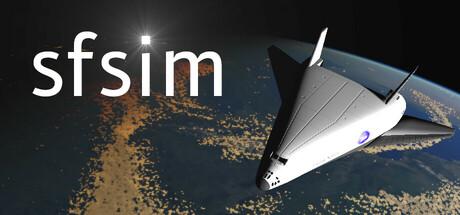
\includegraphics[width=.24\textwidth]{sfsim}
\end{frame}

\begin{frame}
  \pdfbookmark[1]{Inspired by Orbiter 2016}{orbiter}
  \frametitle{Inspired by Orbiter 2016}
  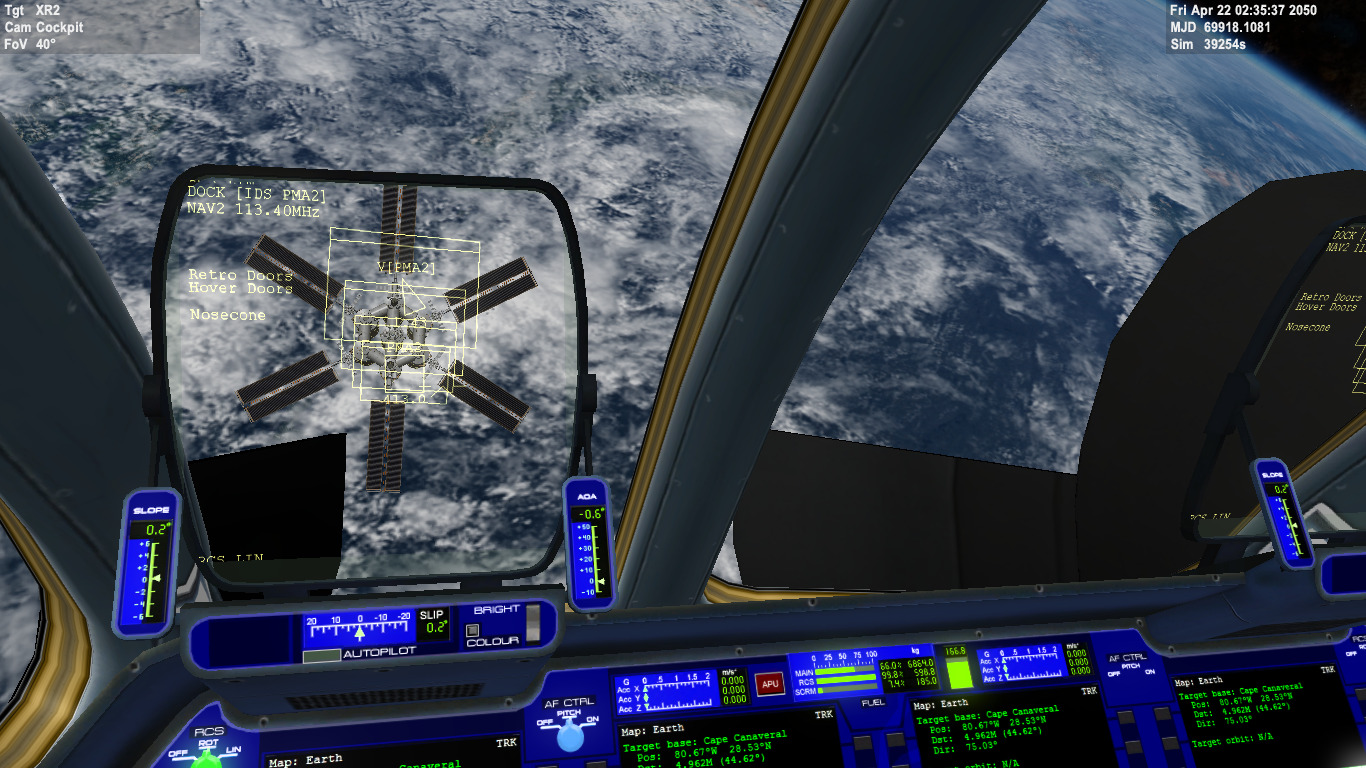
\includegraphics[width=.99\textwidth]{orbiter}
\end{frame}

\begin{frame}
  \pdfbookmark[1]{questions}{questions}
  \begin{center}
    \begin{huge}
      Thanks for listening!
    \end{huge}
  \end{center}
\end{frame}

\end{document}
